\chapter*{\markboth{}{}}  % \markboth{}{} é utilizado para corrigir o cabeçalho.
\phantomsection
\addcontentsline{toc}{chapter}{Dedicatória}
\begin{center}
  \emph{
  % FIXME Remover as duas linhas abaixo.
  Aos meus \ldots. \\
  Para \ldots.} 
\end{center}

\begin{figure}[!htb]
  \center
  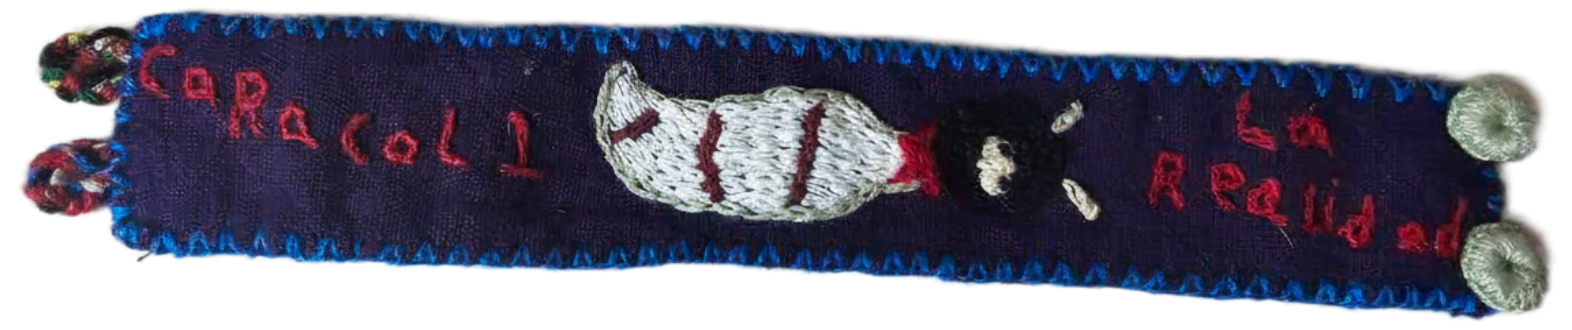
\includegraphics[width=0.8\textwidth]{figuras/caracol_colorido.png}
  \caption*{\textit{Lento, pero avanzo}. Caracol 1, Chiapas, México, dezembro de 2022.}
  \label{fig:scielo_temporal}
\end{figure}

%\begin{figure}[!htb]
 % \center
  %\includegraphics[width=0.8\textwidth]%{figuras/caracol1.png}
  %\caption*{\textit{Lento, pero avanzo}. Caracol 1, %Chiapas, México, dezembro de 2022.}
 % \label{fig:scielo_temporal}
%\end{figure}

%[INSERIR POEMA DE AUTORIA PRÓPRIA SOBRE A VIAGEM AO MÉXICO]

